\documentclass{article}

\usepackage{fancyhdr}
\usepackage{geometry}
\usepackage{chemfig}
\usepackage{amsmath}
\usepackage{pgfplots}
\usepackage{rotating}
\usepackage{multicol}
\usepgfplotslibrary{polar}

\geometry{
    top=20mm,
    bottom=25mm,
    left=20mm,
    right=20mm
}

\pagestyle{fancy}

\renewcommand{\headrulewidth}{0pt}

\fancyfoot[L]{
    \begin{turn}{180}
        \begin{minipage}{0.6\linewidth}
            \flushright
            \begin{multicols}{2}
                \emph{written exclusively under the influence}
                \chemfig{[,0.8]C(-[2]H)(-[4]H)(-[6]H)-H}
            \end{multicols}
        \end{minipage}
    \end{turn}
}

\begin{document}

This shall be a fun exercise. I will need to learn how to produce a tree diagram in \LaTeX{} as well as a TikZ picture of a golden spiral overlaid atop a snail (at the very least).

To accomplish the latter I shall leverage the arc length of a curve as \(\theta_1 \rightarrow \infty\) for \(l\), where

\[ l = \int^{\theta_1}_{\theta_0} \sqrt{[f(\theta)]^2 + [f'(\theta)]^2} \mathrm{d}\theta\]

Then for a given curve such as \(r = e^\frac{\theta}{10}\):
\begin{center} % you could probably tell tikz to center?
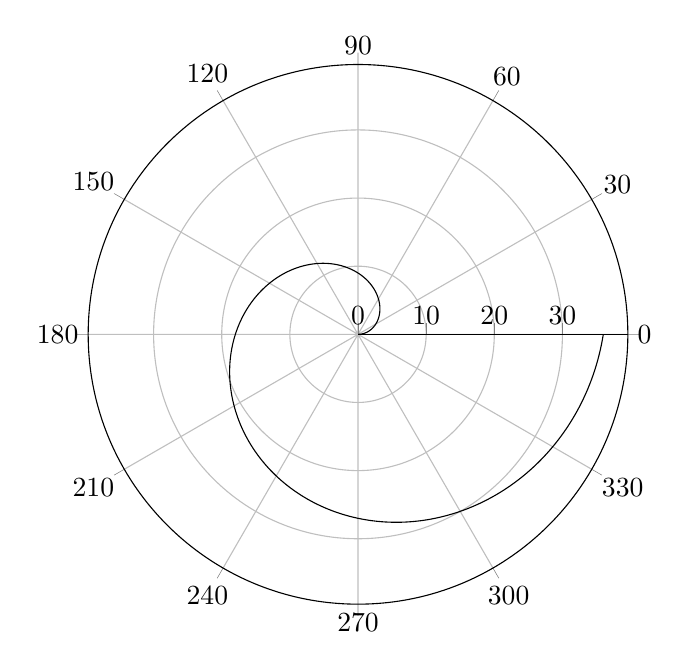
\begin{tikzpicture}
    \begin{polaraxis}
        \addplot[domain=0:360, samples=300]{0.10*x};
    \end{polaraxis}
\end{tikzpicture}
\end{center}

The length of the arc is:
\begin{align*}
    l &= \int^{\theta_1}_{0} \sqrt{(e^{-\frac{\theta}{10}})^2 + (-\frac{1}{10}e^{-\frac{\theta}{10}})^2}\mathrm{d}\theta\\
    &= \int^{\theta_1}_{0} \sqrt{(1+\frac{1}{100})e^{-\frac{2\theta}{10}}} \mathrm{d}\theta\\
    &= \frac{\sqrt{101}}{10} \int^{\theta_1}_0 e^{-\frac{\theta}{10}}\mathrm{d}\theta\\
    &= \sqrt{101}(1 - e^{-\frac{\theta_1}{10}}).\\
    &= \sqrt{101} \text{ (as \(\theta_1 \rightarrow \infty\))}
\end{align*}

\end{document}
